%\documentclass[12pt, twocolumn]{article}
\documentclass[11pt]{article}
\usepackage{amscd} % american math socitey …
\usepackage{amsfonts}
\usepackage{amsmath}
\usepackage{amssymb}
\usepackage{amsthm}
\usepackage{graphicx}
\usepackage{skull}
\usepackage{lipsum}
\usepackage{url}
%\usepackage[
%backend=biber,
%style=alphabetic,
%sorting=ynt
%]{biblatex}
\usepackage{blindtext}
%\addbibresource{hw6.bib}

%adjustments
\parskip=.9ex
%\parindent=1em
\textwidth=7.0in
% \marginparwidth=1.4em
\textheight=9.0in
\oddsidemargin=-.25in
\topmargin=-.75in

\begin{document}

\title{The Wonders of Lorem Ipsum}

\author{Zane Durkin\\
    University of Idaho}

\maketitle

\begin{abstract}
In this article I will be going over the wonders of Lorem Ipsum. I'll be sure to type a majority of the article, but what kind of documentation would be complete without examples? As a common tool in the type setting industry, this tool couldn't be much more appropriate for this assignment. Lorem Ipsum is a dummy text that appears to be normal words when looked at from a glance, and although the tool uses latin, it can often be mistaken for normal english text. I'll be going over practical uses for Lorem Ipsum in the industry, and some example cases in which Lorem Ipsum would be useful.
\end{abstract}

\section{A Tool for the Pros}
\textit{Lorem Ipsum}, A \textbf{common tool} in the type setting industry. Lorem Ipsum is a randomly Generated string of latin words that are specifically chosen to look like a normal language at a glance, and as lipsum.com puts it, ``Lorem Ipsum is simply dummy text of the printing and typesetting industry.~\cite{Lipsum}'' Lorem Ipsum can be a useful tool for designing the layout of an article that you haven't typed yet; It gives the appearance of what your article might look like, so you can make simple design choices before you have to even think about what you're typing about.\\ \indent
But this doesn't come in handy for just the type setting industry, a lot of industries have found practical uses for Lorem Ipsum. As a part time website designer, I have personally found Lorem Ipsum to be very handy when designing the layout of a website. Being able to design the layout of the website can help with determining even how much text will need to be written later on.

\section{Practical Uses}
That's right, it does have a practical use! Not all uses may seem practical for everyone, but if you search enough even random words can be useful for everyone.
\subsection{Where It's Used}
There are many practical uses for Lorem ipsum.
Lets list some out:
\begin{itemize}
\item Getting an estimate on how much text will be needed
\item Filling space to help designers
\item Seeing if someone reads a letter you send them
\item Making an essay you don't want to write
\end{itemize}

\subsection{Places to get it}
Well with so many helpful places to find a generator of Lorem Ipsum, it would be best to given an enumerated list of where they can be found.
\begin{enumerate}
\item https://lipsum.com/
\item Latex even has a couple of packages (Covered in Table~\ref{tbl:dastable})
\item Phython has a package
\item And the all to famous https://baconipsum.com/ (See Figure:~\ref{fig:bacon})
\end{enumerate}
\begin{table}[h]
\centering
\caption{A comparison of \LaTeX\ Lorem Ipsum Packages}
\label{tbl:dastable}
\begin{tabular}{|l|ll|}
\hline
Names & How to call it & Notes \\ \hline
lipsum & \verb=\lipsum[2-7]= & Text is predefined for consistency \\
blindtext & \verb=\blindtext= & Text is randomly Generated each run \\
ptext & \verb=\ptext= & Used for Persian text \\ \hline
\end{tabular}
\end{table}



\section{What Does it Looks Like}
What does Lorem Ipsum look like you might ask, well I'll be happy to generate some.
Here is a single paragraph of Lorem Ipsum as generated by the \verb=\blindtext= package in \LaTeX\ \\
\indent
%\lipsum[4-7]
\blindtext
\begin{figure}[h]
\begin{center}
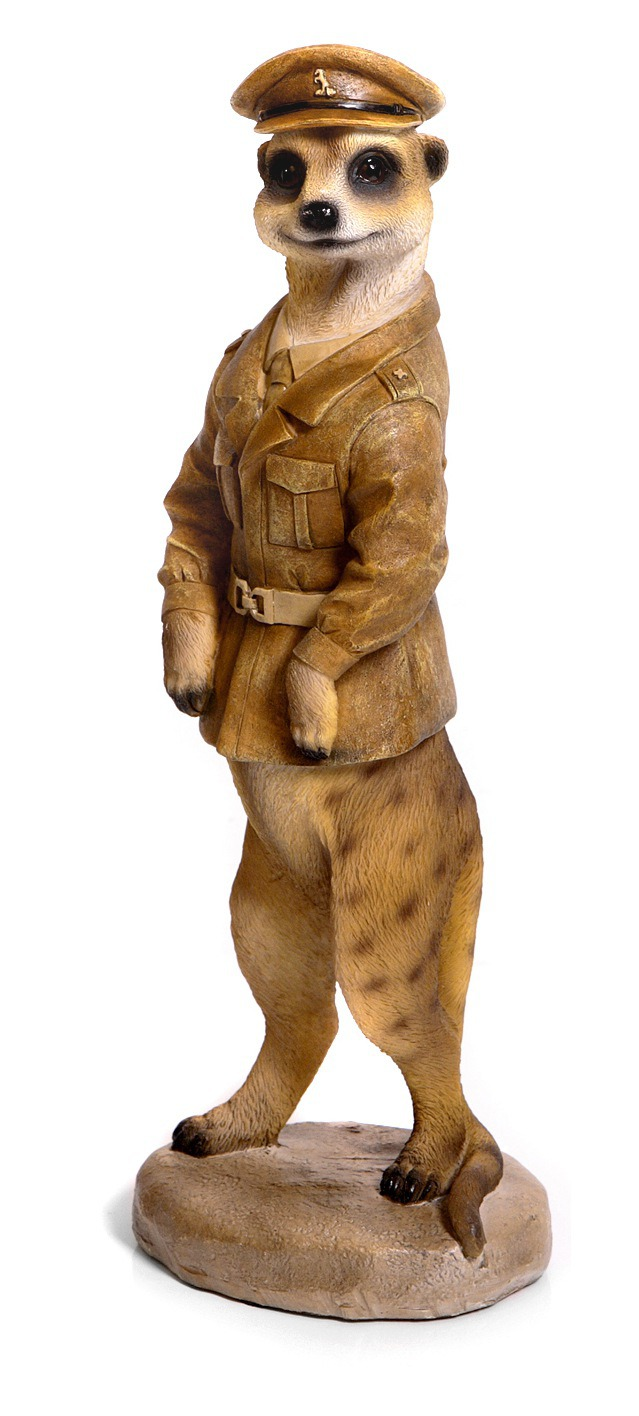
\includegraphics[width=3in, scale=0.5]{captainmeerkat.jpeg}
\end{center}
\caption{A captain meerkat~\cite{meerkat}}
\label{fig:meerkat}
\end{figure}

\begin{figure}
\begin{center}

\includegraphics[width=3in, scale=0.5]{bacon_ipsum.png}
\end{center}
\caption{Bacon Ipsum logo~\cite{bacon}}
\label{fig:bacon}
\end{figure}


\section{Conclusion}
Dogs are great!
Perhaps you may enjoy this image of a meerkat wearing a captain's uniform (See Figure:~\ref{fig:meerkat}).

\section{Math Extras}
\subsection{Four Math Expressions}
Here are four math expressions duplicated
\[
x=\frac{b\pm\sqrt{b^2-4ac}}{2a}
\]
\[
F_{n+1}=F_{n}+F_{n-1}
\]
\[
\Phi(z)=\frac{1}{\sqrt{2\pi}}\int_{0}^z e^{-x^2/2}dx
\]
\[
\sum_{n=1}^{k} n=\frac{k(k+1)}{2}
\]
\subsection{Math Expressions in Align Environment}
\begin{align}
C_n&=\frac{1}{n+1}\binom{2n}{n} \\
&=\frac{(2n)!}{(n+1)!n!} \\
&=\frac{2^n(2n-1)!!}{(n+1)!} \\
&=\left ( \frac{4^n\Gamma(n+\frac{1}{2})}{\sqrt{\pi}\Gamma(n+2)} \right )
\end{align}
\subsection{In-line Math Equations}
Here are some duplicated math expressions:\\
\indent
Morbo the Annihilator is on TV channel $\sqrt{2}$. with Linda van Schoonhoven.\\
\indent
The simple identity is: $e^{\theta i} = \cos{(\theta)} + \sin{(\theta)}i$.
\bibliographystyle{apalike}
\bibliography{hw6}

\end{document}

